\chapter{Experiments and Evaluation}
\label{evaluation}
% DELETEME: The evaluation chapter is one of the most important chapters of your work. Here, you will prove usability/efficiency of your approach by presenting and interpreting your results. You should discuss your results and interpret them, if possible. Drawing conclusions on the results will be one important point that your estimators will refer to when grading your work.

This chapter serves as a presentation of our the dataset used in our experiments, and their output, after which is discussed if it has met the expectations and the approach was efficient in providing a solution for the camera placement optimisation problem.

\section{Experiments}
In this thesis, two different experiments were conducted in order to evaluate the performance loss of cameras. What is more, with the help of heatmaps and using the metrics M1 and M2 we are able to define an optimal camera position. The experiments aim to check if problems from \ref{problem_analysis} are handled efficiently by the proposed strategy. In the next subsections, we inform about the laptop used for our simulations and explain into details each experiment. Afterwards, we discuss the results and the efficiency of our metrics.

\subsection{Technical specifications}
The following list contains technical specifications of the machine, which all experiments were simulated on:
\begin{itemize}
    \item \textbf{Processor} - Intel Core i7-10750H CPU 2.60GHz
    \item \textbf{RAM} - 16 GB DDR5
    \item \textbf{GPU} - NVIDIA GeForce RTX 3060 6 GB
    \item \textbf{SSD} - 1 TB
\end{itemize}

\newpage
\subsection{First experiment - change height and angle of camera}
The main objective of our first experiment is to evaluate the performance of cameras at different height, because we concluded in Chapter \ref{problem_analysis} that in the found literature there is little information about which height is optimal for traffic surveillance. During the execution of simulations, we rely on a camera with the following configurations:
\begin{itemize}
    \item FoV (horizontal angle) = $80^{\circ}$
    \item Resolution = $1280\times720$ pixels or also known as 720p
\end{itemize}
The reason for our horizontal angle is that we wanted to cover as much as possible from our region of interest and an average traffic surveillance camera on the market has a horizontal field of view $70^{\circ} - 110^{\circ}$. In a real-world scenario, a wider field of view will cause a fisheye effect\footnote{When an image is distorted by stretching the picture around a rounded camera lens} to occur and has to be taken into account. However, in our experiments the conditions are ideal and we do not apply image distortion. We have 8 enumerated positions for the camera, which can be seen in Figure \ref{fig:positions_enumerated}, where we place it at a pre-defined height. On each of these spawn locations for our sensor, we define 6 levels for the height beginning at 5 meters and going to 10 meters with a 1-meter step. This results in 48 simulations, where we set $0^{\circ}$ for the tilt angle at 5 meters, $-10^{\circ}$ at 6 meters and then go to $-30^{\circ}$ at 10 meters with a $-5^{\circ}$ step. In this way we guarantee that the camera has approximately the same sight over the vehicles. The region of interest is limited by the red lines in Figure \ref{fig:positions_enumerated} and is used in each of the two experiments.

During each simulation, we generate a list with waypoints for the target vehicle that are 3 meters apart and one for the occluder, but with 1-meter distance between spawn points. We decided to use Seat Leon as a target and Jeep Wrangler Rubicon as an occluder for our scenarios, because in an urban area people mainly use normal cars or SUVs for their transportation needs, and therefore it is more often the case that an occlusion-prone situation between these two types of vehicles arises. In our second experiment we consider pairs of vehicles of different type in order to broaden the variety of occlusions.

\begin{figure} [h!]
    \centering
    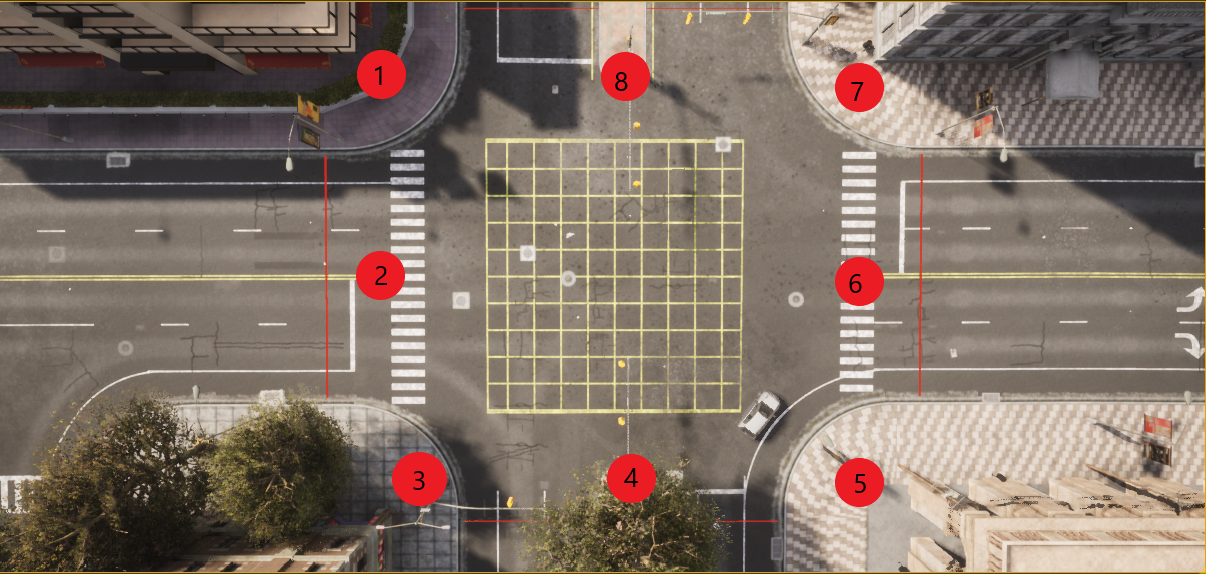
\includegraphics[width=0.90\textwidth]{images/positions_numerated.png}
    \caption[Enumerated camera positions]{This image shows the number of each camera's position used in our simulations.}
    \label{fig:positions_enumerated}
\end{figure}

\subsection{Second experiment - change threshold for target vehicle recognition}

%###################################################################################
%###################### Results             ########################################
%###################################################################################
\section{Results}\label{results}

%###################################################################################
%###################### Discussions         ########################################
%###################################################################################
\section{Discussions}\label{discussions}
\subsection{Results of first experiment}
\subsection{Results of second experiment}
\subsection{Efficiency of metrics}